\documentclass[UTF8,11pt]{ctexart}

\usepackage[a4paper,margin=2.2cm]{geometry}
\usepackage{graphicx}
\usepackage{subcaption}
\usepackage{booktabs}
\usepackage{longtable}
\usepackage{array}
\usepackage{xcolor}
\usepackage{hyperref}
\usepackage{enumitem}

\graphicspath{{review_pack_20260424_baseline/}}
\hypersetup{
  colorlinks=true,
  linkcolor=blue!60!black,
  urlcolor=blue!60!black,
  citecolor=blue!60!black
}
\setlist[itemize]{leftmargin=1.8em,itemsep=0.2em,topsep=0.3em}

\title{IVOCT 钙化分割 Baseline 实验报告}
\author{CN\_seg 实验记录}
\date{2026-04-24}

\begin{document}
\maketitle

\begin{abstract}
本文档整理当前阶段最优的 IVOCT 钙化分割实验。当前正式主线为
\textbf{MAE encoder + Conv decoder} 的 reproduced baseline，在 4 名患者
LOPO-CV 上取得 Mean Dice $0.5212 \pm 0.1424$。阈值扫描显示统一阈值
$0.3$ 仍是当前最合适的全局选择。针对最弱患者 P002 的定向改动虽能改善
该折，但会损害整体 LOPO 表现，因此不作为当前主线。现阶段建议停止围绕
现有 4 名患者继续过度调参，等待剩余 14 名患者数据到位后重新评估泛化能力。
\end{abstract}

\section{实验策略}

当前最优实验采用冻结 MAE encoder、训练 Conv decoder 的分割方案。验证方式为
leave-one-patient-out cross validation (LOPO-CV)，每一折保留 1 名患者作为验证集，
其余患者用于训练。

\begin{table}[htbp]
\centering
\caption{当前主线实验配置}
\begin{tabular}{ll}
\toprule
项目 & 配置 \\
\midrule
模型 & MAE encoder + Conv decoder \\
训练方式 & LOPO-CV \\
输入尺寸 & $256 \times 256$ \\
ROI 裁剪比例 & 0.86 \\
Encoder & 冻结 \\
Decoder 学习率 & $1 \times 10^{-3}$ \\
评估阈值 & 0.3 \\
训练脚本 & \texttt{seven/seg/train\_seg.py} \\
服务器运行目录 & \texttt{/root/CN\_seg\_baseline/seven/seg} \\
\bottomrule
\end{tabular}
\end{table}

\section{主线结果}

当前最优主线结果来自 baseline 重跑，结果文件为：

\begin{center}
\texttt{/root/CN\_seg\_baseline/seven/seg/logs/results\_lopo\_20260424\_004401.json}
\end{center}

整体结果为 Mean Dice $0.5212 \pm 0.1424$。分折结果见表~\ref{tab:fold-results}。

\begin{table}[htbp]
\centering
\caption{Baseline LOPO-CV 分折结果}
\label{tab:fold-results}
\begin{tabular}{ccccc}
\toprule
Fold & 验证患者 & Best Epoch & Dice Mean & IoU Mean \\
\midrule
0 & P001 & 177 & 0.5288 & 0.3746 \\
1 & P002 & 168 & 0.2861 & 0.1805 \\
2 & P003 & 52  & 0.6323 & 0.4643 \\
3 & P004 & 94  & 0.6374 & 0.4775 \\
\midrule
\multicolumn{3}{r}{Mean $\pm$ Std} & $0.5212 \pm 0.1424$ & -- \\
\bottomrule
\end{tabular}
\end{table}

P002 是当前 4 名患者中最弱的一折。后续分析表明，该折存在明显的患者间泛化波动；
但在现有 4 名患者规模下，继续只针对 P002 调整全局配置会引入过拟合风险。

\section{可视化结果}

图~\ref{fig:fold-vis} 展示了每一折 best epoch 对应的分割可视化。每张图中包含输入图像、
模型预测与人工标注的对照。

\begin{figure}[htbp]
\centering
\begin{subfigure}{0.48\textwidth}
  \centering
  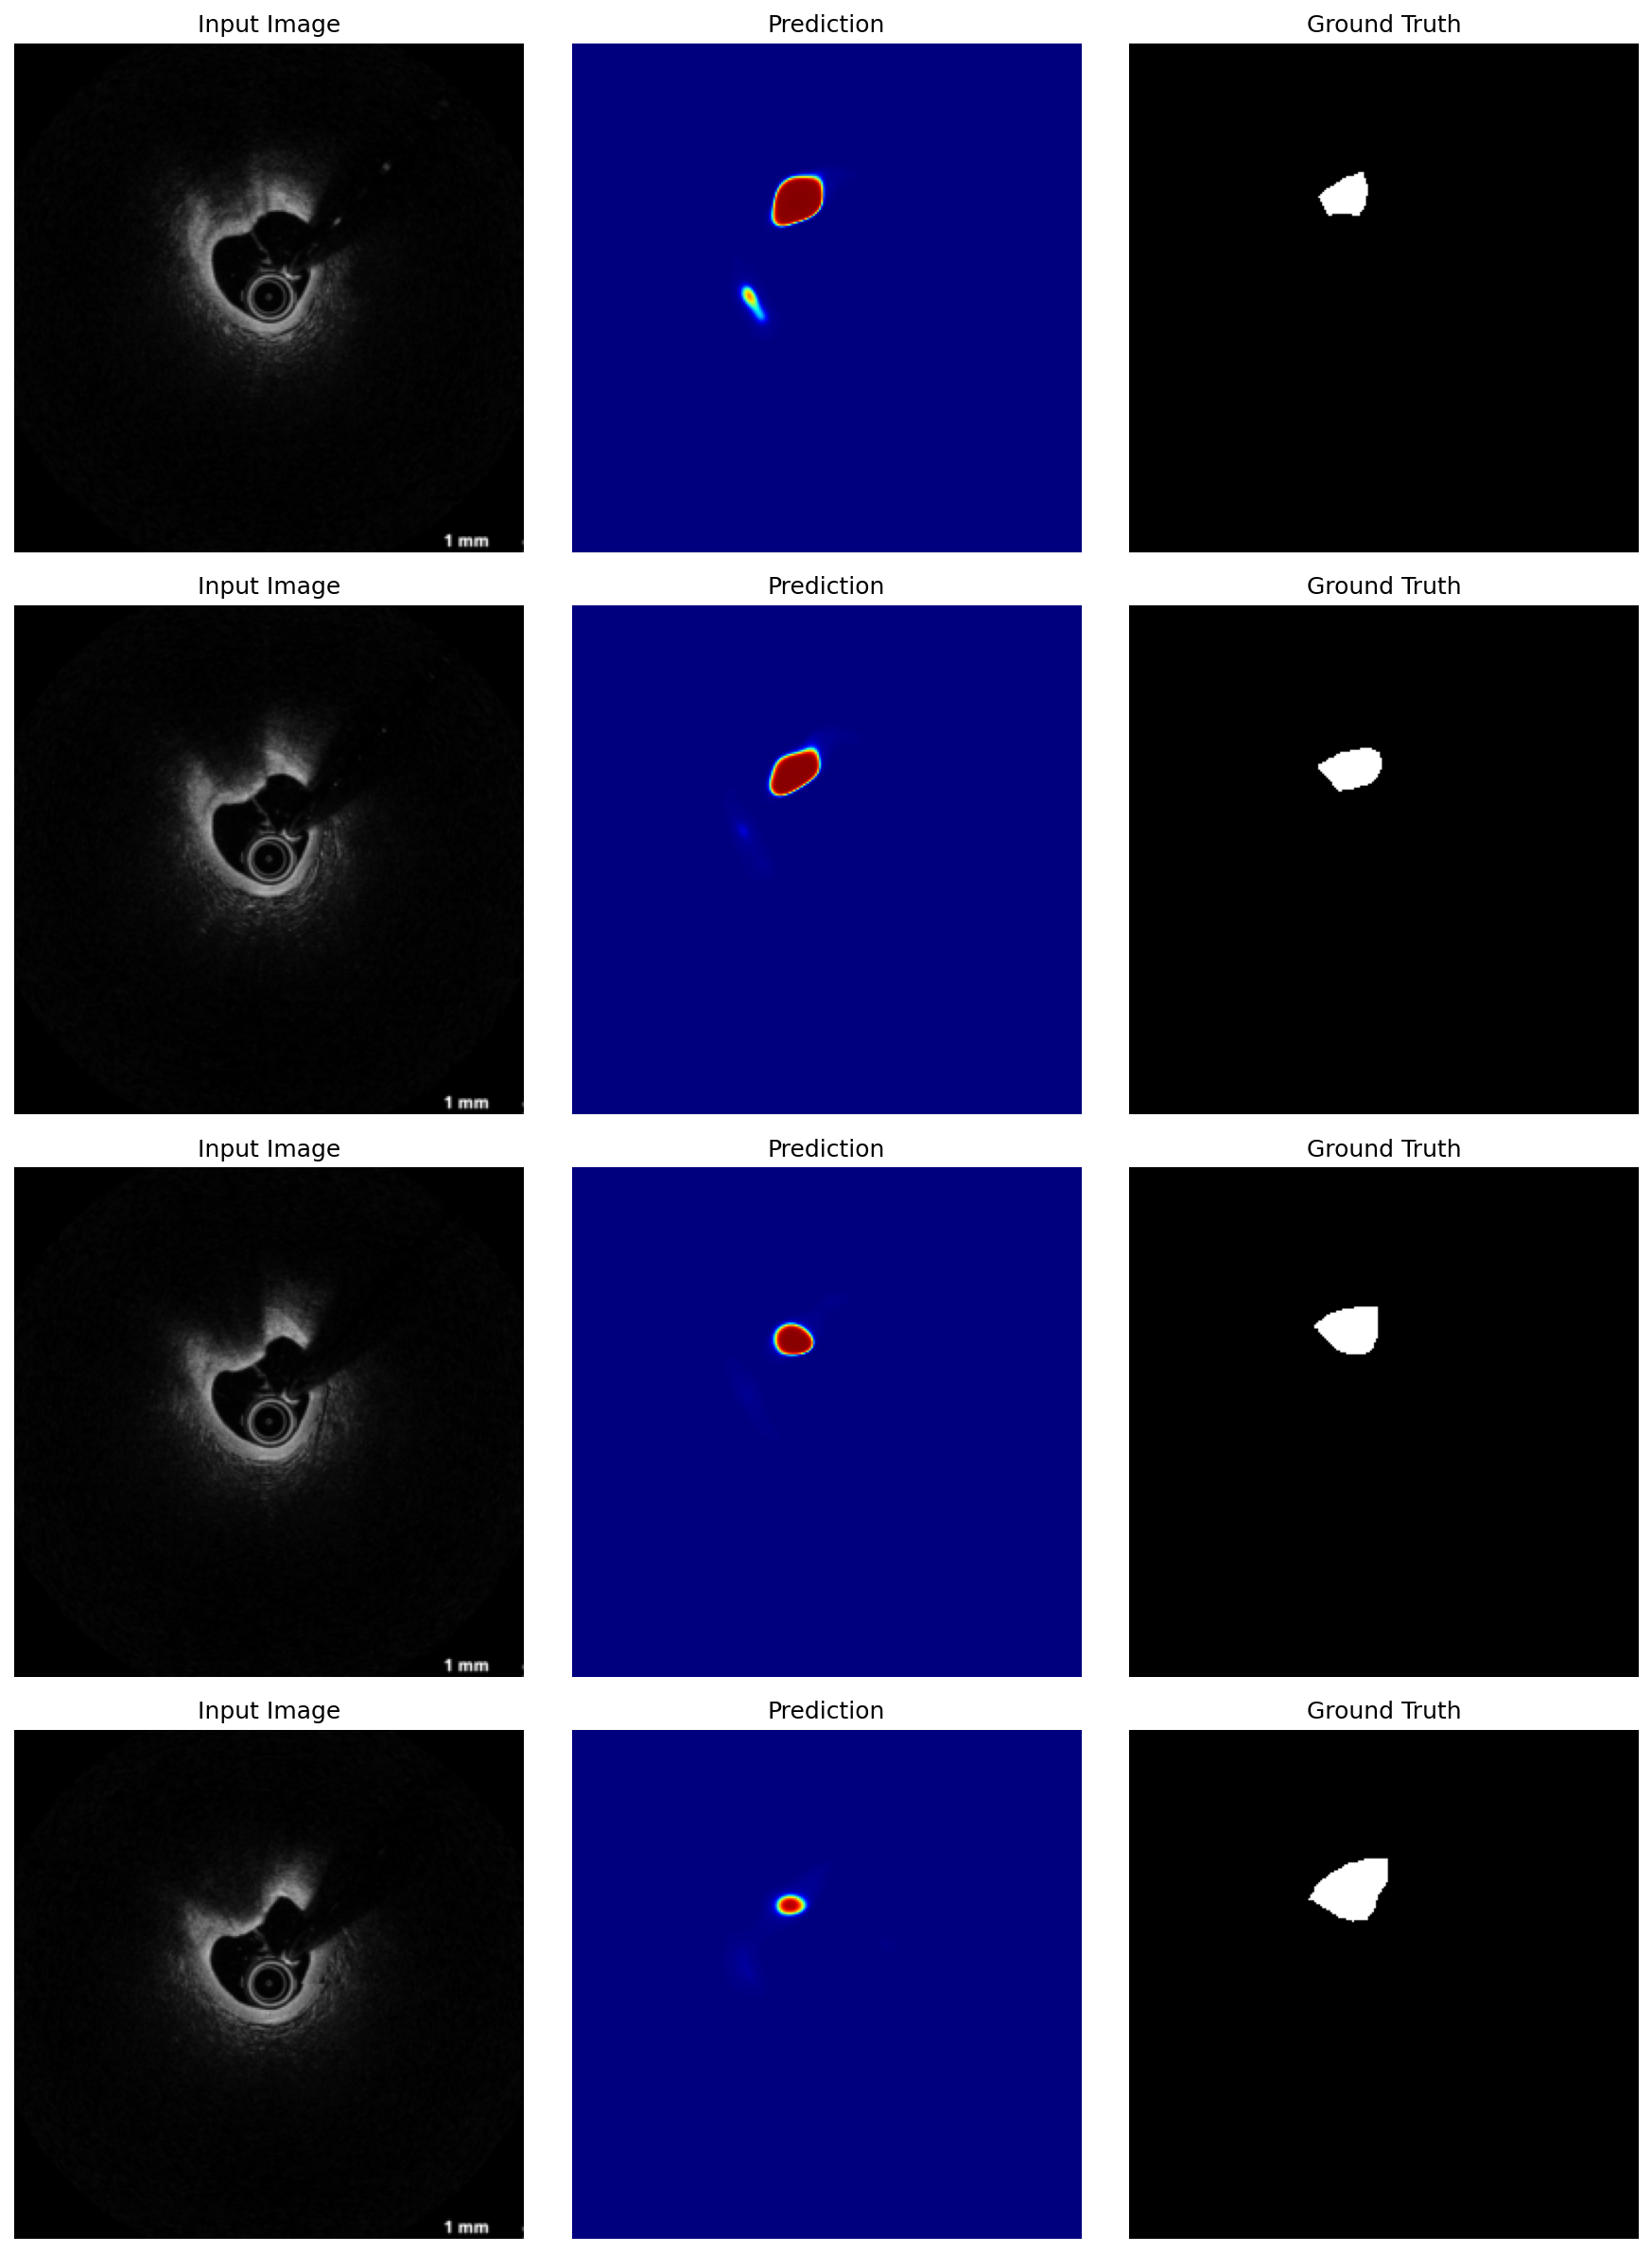
\includegraphics[width=\linewidth]{fold_0_best_epoch_177.png}
  \caption{Fold 0, val=P001, Dice=0.5288}
\end{subfigure}
\hfill
\begin{subfigure}{0.48\textwidth}
  \centering
  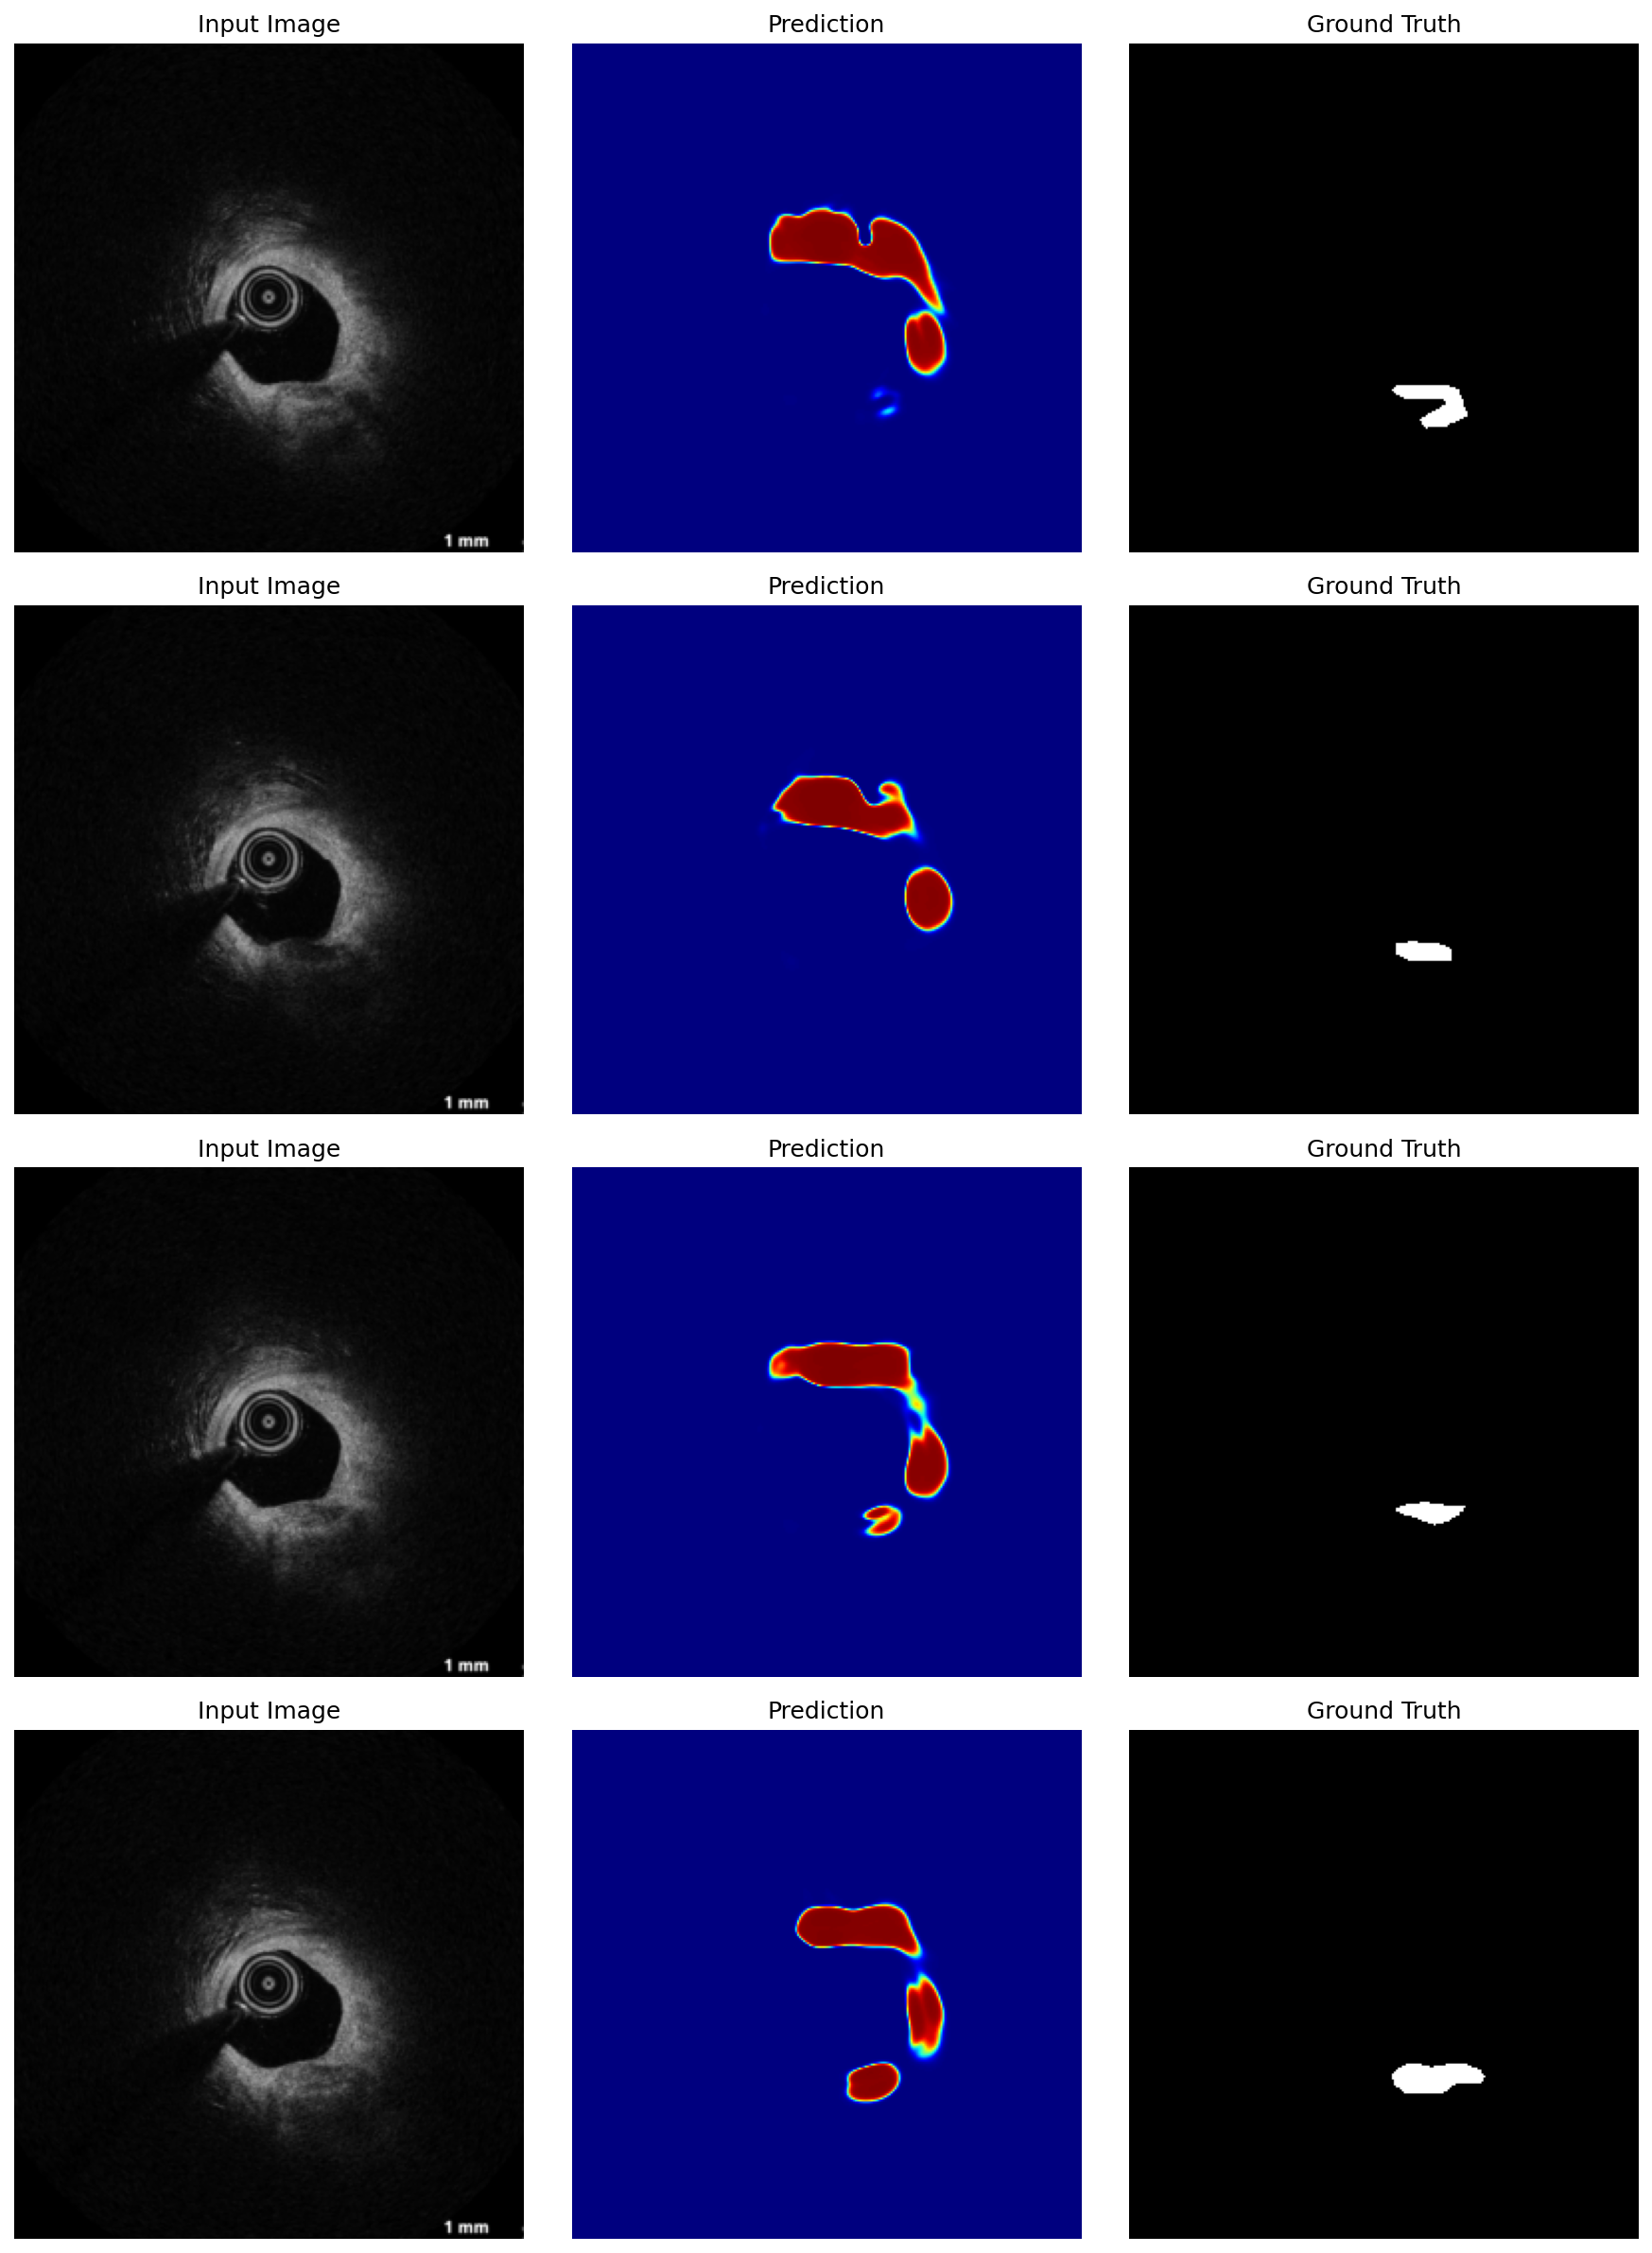
\includegraphics[width=\linewidth]{fold_1_best_epoch_168.png}
  \caption{Fold 1, val=P002, Dice=0.2861}
\end{subfigure}

\vspace{0.8em}

\begin{subfigure}{0.48\textwidth}
  \centering
  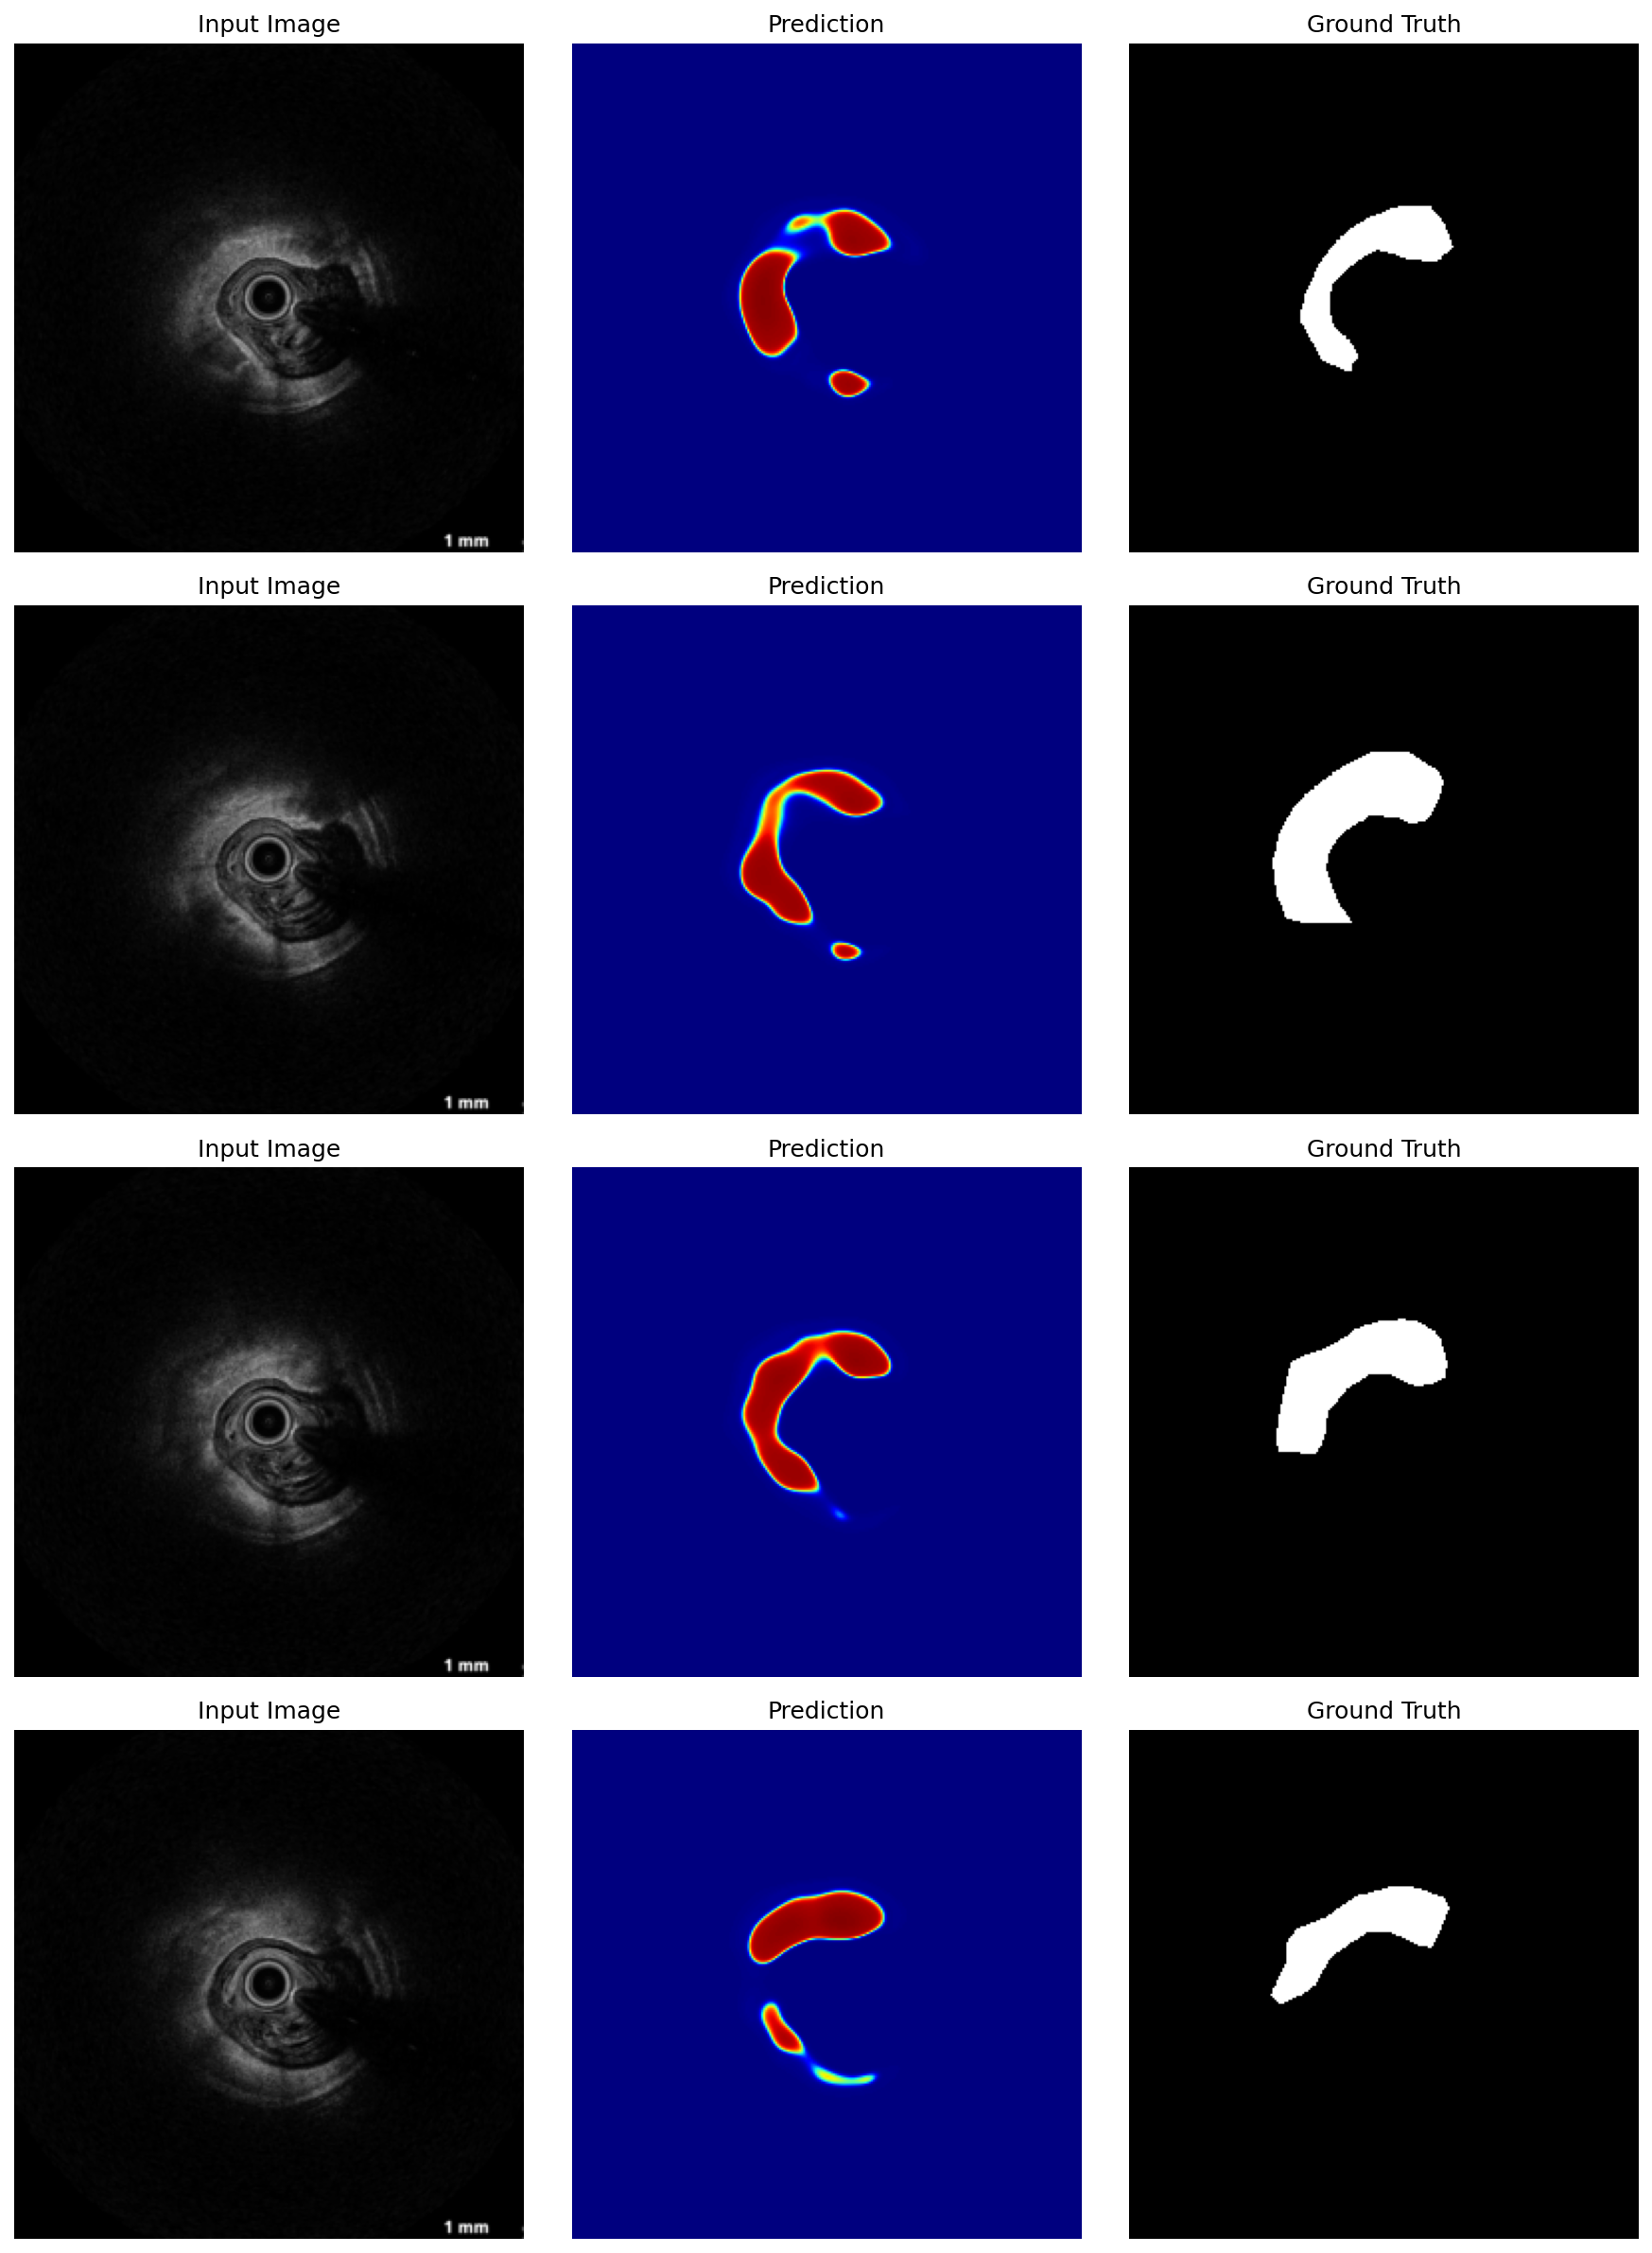
\includegraphics[width=\linewidth]{fold_2_best_epoch_052.png}
  \caption{Fold 2, val=P003, Dice=0.6323}
\end{subfigure}
\hfill
\begin{subfigure}{0.48\textwidth}
  \centering
  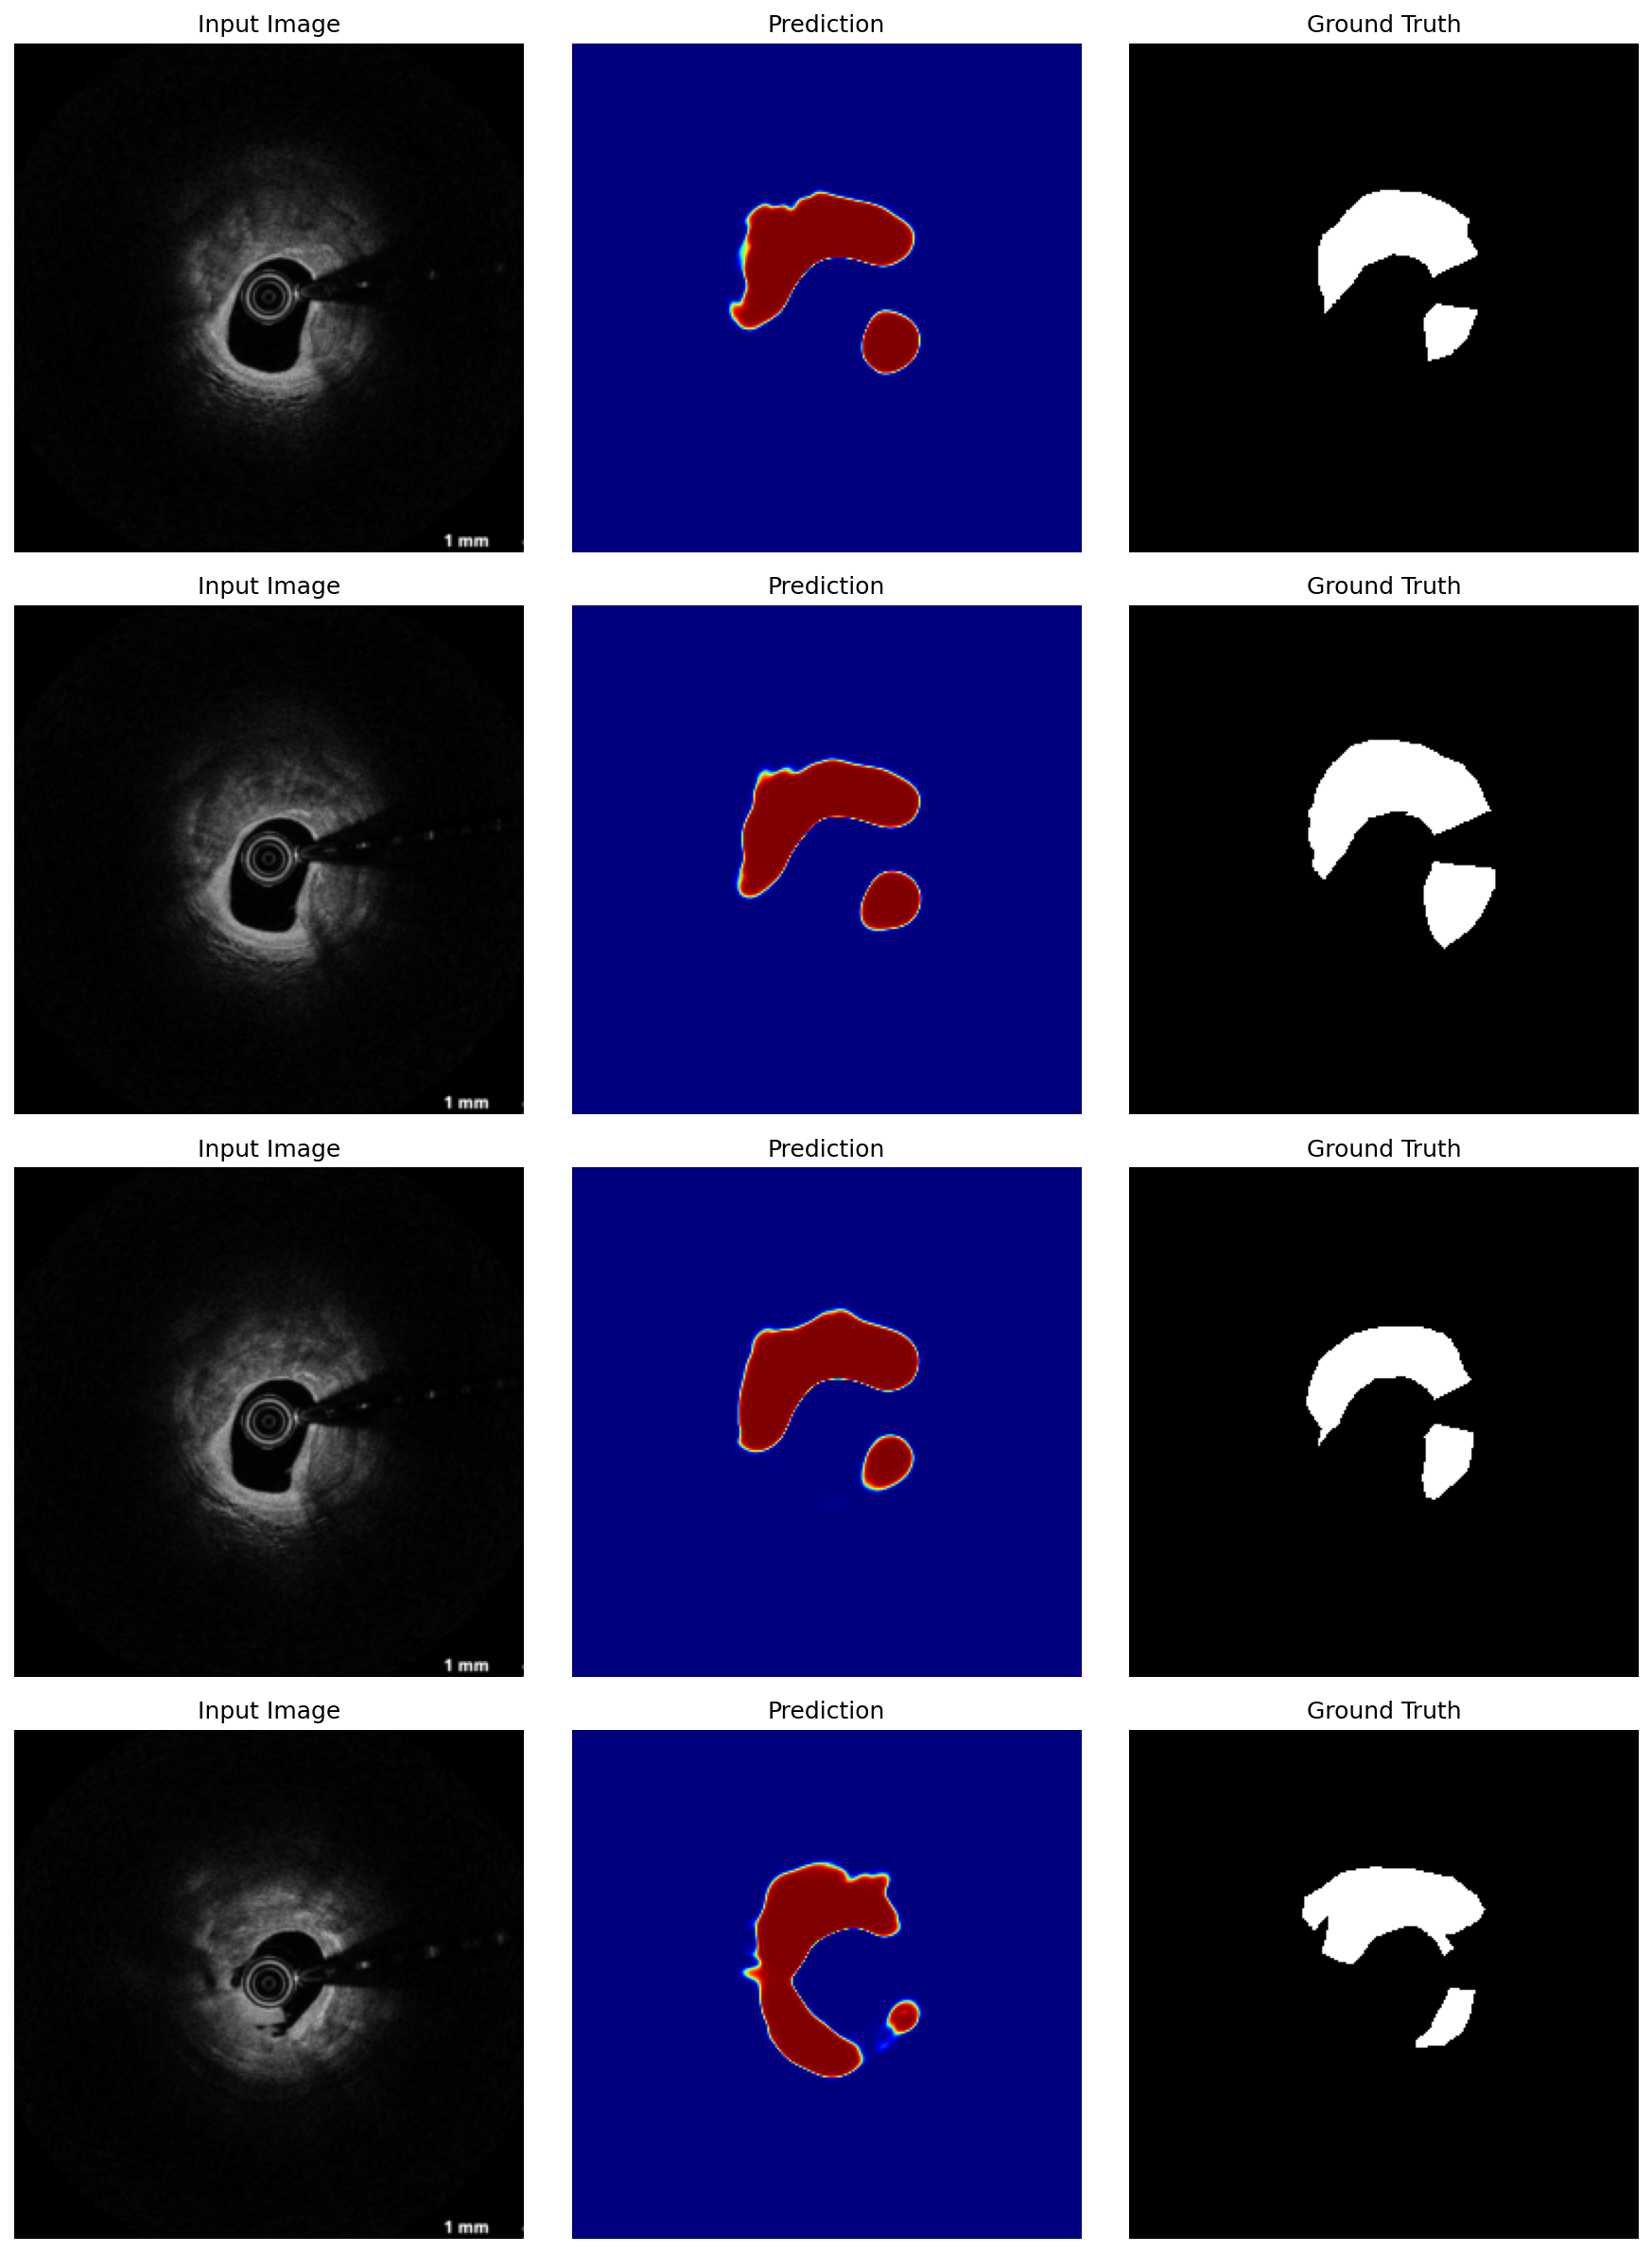
\includegraphics[width=\linewidth]{fold_3_best_epoch_094.png}
  \caption{Fold 3, val=P004, Dice=0.6374}
\end{subfigure}
\caption{Baseline 各 fold 的 best epoch 可视化结果。}
\label{fig:fold-vis}
\end{figure}

\section{阈值扫描}

对 reproduced baseline checkpoints 进行阈值扫描后，全局最优统一阈值仍为 0.3，
对应 Mean Dice 为 0.5213。阈值扫描没有带来实质性的全局提升，因此当前主线继续使用
0.3 作为统一评估阈值。

\begin{table}[htbp]
\centering
\caption{阈值扫描中的每折最优阈值}
\begin{tabular}{cccc}
\toprule
Fold & 验证患者 & 单折最优阈值 & 单折最优 Dice \\
\midrule
0 & P001 & 0.3 & 0.5292 \\
1 & P002 & 0.7 & 0.2895 \\
2 & P003 & 0.3 & 0.6323 \\
3 & P004 & 0.6 & 0.6384 \\
\midrule
\multicolumn{2}{r}{全局统一最优阈值} & 0.3 & 0.5213 \\
\bottomrule
\end{tabular}
\end{table}

需要注意的是，P002 的单折最优阈值为 0.7，但 Dice 仅从 0.2864 提升到 0.2895，
说明 P002 的主要问题不是简单的阈值校准，而是患者间泛化与结构性误分割。

\section{已验证但未采用的方案}

围绕 P002 的误差模式，已经验证过几类定向方案。它们对 P002 可能有局部改善，
但不能成为当前全局主线。

\begin{table}[htbp]
\centering
\caption{未采用方案及原因}
\begin{tabular}{p{0.28\textwidth}p{0.22\textwidth}p{0.38\textwidth}}
\toprule
方案 & 结果 & 结论 \\
\midrule
全局连通域后处理 & P002 提升，但 P003/P004 明显下降 & 不适合做统一后处理 \\
Focal alpha=0.5 & P002 Dice=0.2762 & 低于 baseline 的 0.2861 \\
BN + early stopping & P002 Dice=0.2409 & 明显低于 baseline \\
Focal Tversky + BN + early stopping & P002 LOPO Dice=0.3223，全局 Mean Dice=0.4561 & 改善 P002，但损害 P001/P003，全局低于 baseline \\
\bottomrule
\end{tabular}
\end{table}

\section{结果文件索引}

\begin{longtable}{p{0.25\textwidth}p{0.68\textwidth}}
\caption{本报告引用的关键文件}\\
\toprule
类型 & 路径 \\
\midrule
\endfirsthead
\toprule
类型 & 路径 \\
\midrule
\endhead
Review pack 压缩包 & \texttt{result/review\_pack\_20260424\_baseline.tar.gz} \\
Review pack 解压目录 & \texttt{result/review\_pack\_20260424\_baseline/} \\
服务器最优结果 JSON & \texttt{/root/CN\_seg\_baseline/seven/seg/logs/results\_lopo\_20260424\_004401.json} \\
本地 checkpoint 摘要 & \texttt{result/review\_pack\_20260424\_baseline\_checkpoint\_summary.json} \\
本地阈值扫描摘要 & \texttt{result/threshold\_sweep\_summary\_20260424\_baseline.json} \\
Fold 0 可视化 & \texttt{result/review\_pack\_20260424\_baseline/fold\_0\_best\_epoch\_177.png} \\
Fold 1 可视化 & \texttt{result/review\_pack\_20260424\_baseline/fold\_1\_best\_epoch\_168.png} \\
Fold 2 可视化 & \texttt{result/review\_pack\_20260424\_baseline/fold\_2\_best\_epoch\_052.png} \\
Fold 3 可视化 & \texttt{result/review\_pack\_20260424\_baseline/fold\_3\_best\_epoch\_094.png} \\
决策记录 & \texttt{result/seg\_best\_decision\_20260424.md} \\
\bottomrule
\end{longtable}

\section{当前决策}

当前阶段建议保留 reproduced baseline 作为正式 baseline，并暂停围绕现有 4 名患者继续
深挖训练配置。下一阶段应等待剩余 14 名患者数据到位后，再重新进行 patient-level
泛化评估、LOPO-CV 和必要的 loss/采样策略调整。

\end{document}
